% -------------------------------------------------------------------------------------------------
% INTRODUCTION
% -------------------------------------------------------------------------------------------------
\section{Introduction}
\label{sec:introduction}
In recent years, computing is becoming more ubiquitous in the physical world. This
notion where computational elements are embedded seamlessly in ordinary objects that
are connected through a continuous network was introduced many years ago\cite{weiser1991computer}.
The progress towards ubiquitous computing has been slower than expected, technology advances such
as the mobile Internet contributes to achieve this vision in which individual devices are
able to communicate between themselves from any part of the world\cite{gubbi2013internet}. Recently,
this ubiquitous world is close to becoming reality thanks to the Internet of Things and Cloud Computing
\cite{caceres2012ubicomp}. In this vision, physical items are continuously connected to the virtual
world and can act as remotely physical access points to Internet Services\cite{mattern2010internet}.

A common scenario where the Internet of Things paradigm is applied are smart places \cite{atzori2010internet}.
Smart places are an ecosystem composed of sensors - e.g. RFID tags - actuators - e.g. automatic doors -
and computing infrastructure - e.g. cloud servers - that are able to acquire data about the surrounding
environment and use that data to improve the experience of the people using the place \cite{cook2004smart}.

The smart place life-cycle is composed of several stages, starting from the installation of sensors and
readers in the smart place, provisioning the computing infrastructure of the smart place, upload the events
that occur in the physical world to the servers, monitoring the quality of service (\textit{QoS}) of the smart
place and eventually deprovisioning the computing infrastructure, as illustrated on Figure
\ref{fig:smartplace_lifecycle}.

% Smart place life cycle
\begin{figure}
  \centering
  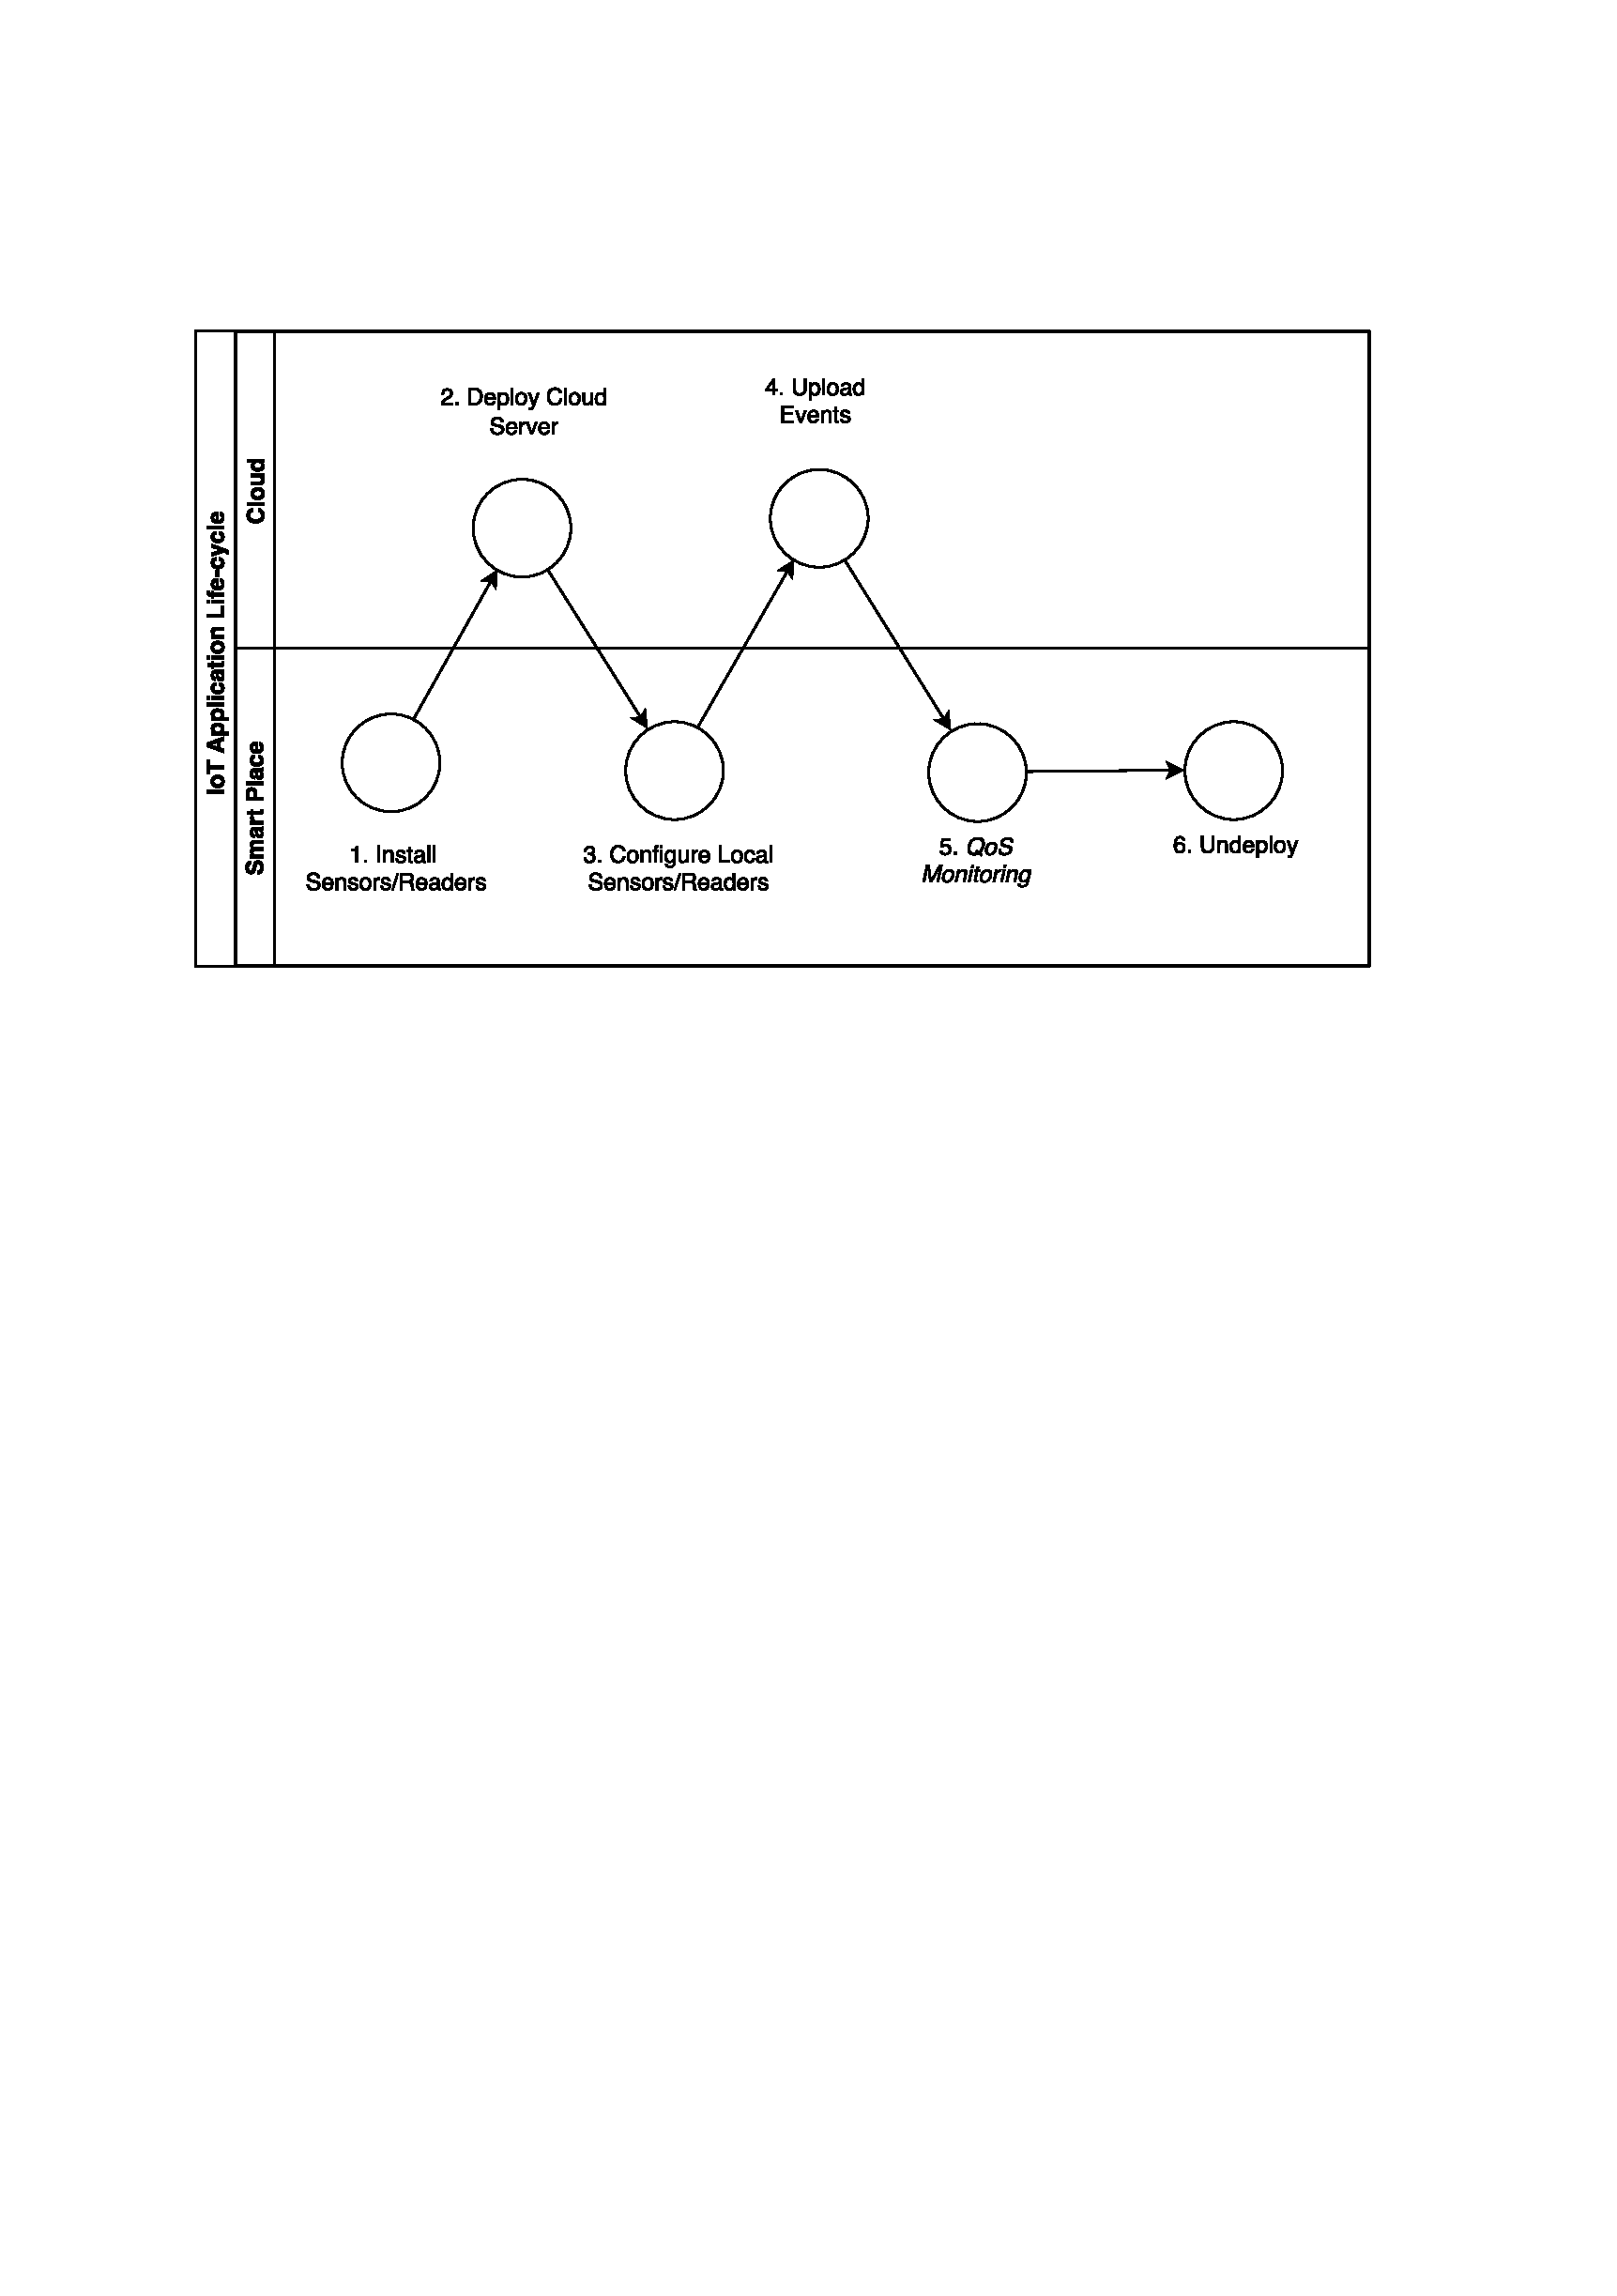
\includegraphics[width=\textwidth]{images/life-cycle.pdf}
  \caption{Smart place life-cycle.}
  \label{fig:smartplace_lifecycle}
\end{figure}

An example of a smart place is a smart warehouse. In the smart warehouse, products and objects
are identified with RFID tags. The data transmitted by the tags is consumed by the computing
infrastructure of the warehouse and then transformed into information. For instance,
Fosstrak\footnote{ Fosstrak is a complete example of a platform that can be used to transform
the RFID data into information, since that implements most of the EPC Network standards.} can use
this information to determine the objects that enter and leaves the smart warehouse.

The smart place infrastructure is divided essentially into two components: the infrastructure in location -
the readers, sensors, power, network connection - and the computing infrastructure - servers, database.
Is not practical the allocation of the physical infrastructure in the smart place itself. This makes the smart place
cost ineffective, since there is a substantial increase in the resource consumption such as power and network
connection, and also limits the scalability of the smart place. To solve those problems, an alternative is to
allocate the computing infrastructure in the cloud. However, provisioning the computing infrastructure in
the cloud still is a manual process that requires considerable effort and expertise
to be executed.

In order to solve those problems we propose Cloud4Things, a solution that automates a set of stages of the smart
place life-cycle, namely the provisioning of the computing infrastructure in the cloud by relying on configuration
management tools that leverage existing cloud stacks. With Cloud4Things we want to support the life-cycle of smart place
applications, from the initial provisioning to day-to-day operations.

\subsection{Overview}
\label{sub:overview}
The remainder of this paper is organized as follows. In Section \ref{sec:related_work} we
present the related work in the area. Section \ref{sec:solution} presents a description of our
solution architecture and the current implemented prototype. In Section \ref{sec:evaluation}
we will perform a qualitative evaluation and compare our solution with the current approaches to provisioning
a smart place infrastructure. Section \ref{sec:conclusion} presents the conclusion of this paper.
